\classheader{2018-08-22}
Back to $\vec{x}' = A_{2x2} \vec{x}$ in the case where the 2 eigenvalues of $A, \Gamma_1, \Gamma_2$ are real and distinct: $\Gamma_1 \neq \Gamma_2$\\
\textbf{Some Notes: }
\begin{enumerate}[label=\protect\circled{\arabic*}]
	\item This works fine when 0 is an eigenvalue
	\begin{example-N}
		$\vec{x}' = \begin{bmatrix}
			3 & -3\\
			1 & -1
		\end{bmatrix} \vec{x}$. Here characteristic equation is $\Gamma^2 - 2\Gamma = 0$, w/ solutions $\Gamma_1 = 0$, $\Gamma_2 = 2$.\\
		For $\Gamma_1 = 0$, $\vec{v_1} = \begin{bmatrix}
			1\\1
		\end{bmatrix}$ is a choice of eigenvector\\
		For $\Gamma_2 = 2$, $\vec{v_2} = \begin{bmatrix}
			3\\1
		\end{bmatrix}$ is one choice\\
		Then $\vec{x}(t) = c_1\vec{v_1}e^{\Gamma_1 t} + c_2\vec{v_2}e^{\Gamma_2 t} = \boxed{c_1 \begin{bmatrix}
			1\\1
		\end{bmatrix} + c_2 \begin{bmatrix}
			1\\1
		\end{bmatrix} e^{2t}}$ is general solution.
	\end{example-N}
	\textbf{Question:} So what does the phase portrait look like here?
	\begin{center}
		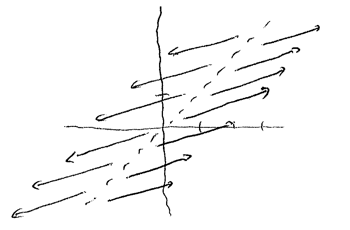
\includegraphics{24-1}
	\end{center}
	\item This formulation of the general solution still works even for repeated eigenvalues \underline{if}	 there are enough eigenvectors.
	\begin{example-N}
		$\vec{x}' = \begin{bmatrix}
			1 & 0 \\ 0 & 1
		\end{bmatrix} \vec{x}$. Here characteristic equation is $\Gamma^2 - 2\Gamma + 1 = 0 = (\Gamma - 1)^2$. Hence $\Gamma_1 = \Gamma_2 = 1$.\\
		The eigenvector equation $\begin{bmatrix}
			1 & 0 \\ 0 & 1
		\end{bmatrix} \begin{bmatrix}
			x_1 \\ x_2
		\end{bmatrix} = 1 \begin{bmatrix}
			x_1\\x_2
		\end{bmatrix}$\\
		One choice is $\vec{v_1} = \begin{bmatrix}
			1 \\ 0 
		\end{bmatrix}, \vec{v_2} = \begin{bmatrix}
			0 \\ 1
		\end{bmatrix}$
		\begin{equation*}
			\text{Hence } \vec{x}(t) = c_1 \begin{bmatrix}
			1 \\ 0 
		\end{bmatrix} e^t + c_2 \begin{bmatrix}
			0 \\ 1 
		\end{bmatrix} e^t \text{ is the general solution}
		\end{equation*} 
	\end{example-N}
	\begin{example-N}
		$\vec{x}' = \begin{bmatrix}
			0 & 1 & 1\\
			1 & 0 & 1\\
			1 & 1 & 0
		\end{bmatrix} \vec{x}$\\
		Here $A = \begin{bmatrix}
			0 & 1 & 1\\
			1 & 0 & 1\\
			1 & 1 & 0
		\end{bmatrix}$ and the characteristic equation after $\det (A - \Gamma I)$ is $\boxed{(\Gamma + 1)^2 (\Gamma -2)}$. The eigenvalues are $\Gamma_1 = 2$, $\Gamma_2 = \Gamma_3 = -1$\\
		The respective eigenvectors are
		$\vec{v_1} = \begin{bmatrix}
			1\\1\\1
		\end{bmatrix}$, $\vec{v_2} = \begin{bmatrix}
			1\\0\\-1
		\end{bmatrix}$, $\vec{v_3} = \begin{bmatrix}
			0\\1\\-1
		\end{bmatrix}$\\
		So the general solution is 
		\begin{equation*}
			\vec{x}(t) = c_1 \begin{bmatrix}
			1\\1\\1
		\end{bmatrix} e^{2t} + c_2 \begin{bmatrix}
			1\\0\\-1
		\end{bmatrix} e^{-t} + c_3
		\begin{bmatrix}
			0\\1\\-1
		\end{bmatrix} e^{-t}
		\end{equation*}
	\end{example-N}
	\item  This formulation for finding solution \underline{does not} work when there are not enough independent eigenvectors for repeated eigenvalues
	\begin{example-N}
		$\vec{x}' = \begin{bmatrix}
			-2 & 1\\
			0 & -2
		\end{bmatrix} \vec{x}$. Here eigenvalues are $\Gamma_1 = \Gamma_2 = -2$. But the eigenvector equation $A\vec{v} = -2\vec{v}$, or
		\begin{align*}
			-2x_1 + x_2 & = -2x_2\\
			-2x_2 & = -2x_2
		\end{align*}
		is \underline{only} solved by $x_2 = 0$, $x_2 \neq 0$. Then only independent choice would be $\vec{v} = \begin{bmatrix}
			1\\0
		\end{bmatrix}$\\
	\end{example-N}
	Here, we will need to come up with another method to find another independent solution.
\end{enumerate}
\subsubsection*{Properties of phase portraits}
let $\vec{x}' = A\vec{x}$. We have
\begin{enumerate}[label=\protect\circled{\arabic*}]
	\item For \underline{any} $A_{2x2}$, the origin is an equilibrium solution ($\vec{x} = \begin{bmatrix}
		0\\0
	\end{bmatrix}$ is always a solution to $A\vec{x} = \vec{0}$).
	\item If $\det A \neq 0$, then $\vec{x} = \begin{bmatrix}
		0\\0
	\end{bmatrix}$ is the \underline{ONLY} equilibrium solution (\underline{stationary point}, or \underline{fixed point}), since $A\vec{x} = \vec{0}$ has $\begin{bmatrix}
		0\\0
	\end{bmatrix}$ as the only solution.
	\item The eigenvectors of $A$ correspond to lines through the origin where the solutions exhibit straight line motion\\
	\textbf{Note: } These straight lines contain many distinct solutions.
	\item The sign of each eigenvalue determines direction along lines (towered origin if $<0$ outward if $>0$).
	\item If eigenvalues are real and distinct then there are the only straight lines (why?)
	\item Signs of eigenvalues determine "stability" of equilibrium at origin. (How solutions behave "near" the origin. Do they stay nearby, converse to, or diverse from...)
	\item Below, origin is called a \underline{"saddle point"} . Would you consider it saddle?
\end{enumerate}
\begin{example-N}
	$\vec{x} = \begin{bmatrix}
		-4 & 1\\
		3 & -2
	\end{bmatrix} \vec{x} \quad \quad$ Here $\Gamma_1 = -5, \Gamma_2 = -1$, with $\vec{v}_1 = \begin{bmatrix}
		-1 \\1
	\end{bmatrix}, \vec{v}_2 = \begin{bmatrix}
		1 \\3
	\end{bmatrix}$\\
	General solution is $\vec{x}(t) = c_1 \begin{bmatrix}
		-1 \\1
	\end{bmatrix} e^{-5t} + c_2 \begin{bmatrix}
		1 \\3
	\end{bmatrix} e^{-t}$. Phase portrait is similar to above but different: how?\\
	Here origin is a "sink" and asymptotically stable.
	\begin{center}
		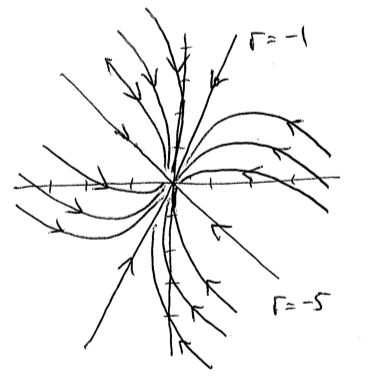
\includegraphics[scale=0.6]{24-2}
	\end{center}
\end{example-N}
\begin{example-N}
	$\vec{x} = \begin{bmatrix}
		1 & 0\\
		0 & 1
	\end{bmatrix} \vec{x} \quad \quad$ Here, as we have seen $\Gamma_1 = \Gamma_2 = 1$, $\vec{v_1} = \begin{bmatrix}
		1\\0
	\end{bmatrix}, \vec{v_2} = \begin{bmatrix}
		0\\1
	\end{bmatrix}$ and General solution is $\vec{x}(t) = c_1 \begin{bmatrix}
		1\\0
	\end{bmatrix}e^t + c_2 \begin{bmatrix}
		0\\1
	\end{bmatrix} e^t = \bigg( c_1 \begin{bmatrix}
		1\\0
	\end{bmatrix} + c_2 \begin{bmatrix}
		0\\1
	\end{bmatrix} \bigg)e^t$.\\
	This is another sources at the origin hhere called a \underline{star node}
	\begin{center}
		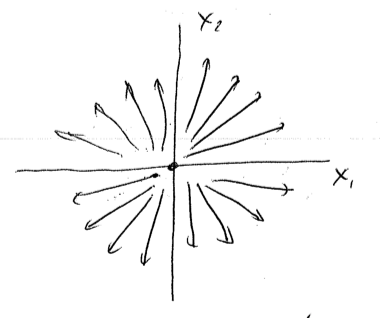
\includegraphics[scale=0.7]{24-3}
	\end{center}
\end{example-N}
\begin{example-N}
	$\vec{x} = \begin{bmatrix}
		3 & -3\\
		1 & -1
	\end{bmatrix} \vec{x} \quad \quad$ Here $\Gamma_1 = 0, \Gamma_2 = 2$, $\vec{v_1} = \begin{bmatrix}
		1\\1
	\end{bmatrix}, \vec{v_2} = \begin{bmatrix}
		3\\1
	\end{bmatrix}$ and General solution is $\vec{x}(t) = c_1 \begin{bmatrix}
		1\\2
	\end{bmatrix} + c_2 \begin{bmatrix}
		3\\1
	\end{bmatrix} e^{2t}$\\
	This one is special: There is a line of equilibrium solution (determinant is 0). Off the dotted line, motion is straight along lines parallel to $\begin{bmatrix}
		3\\1
	\end{bmatrix}$ and moving out from dotted line.
	\begin{center}
		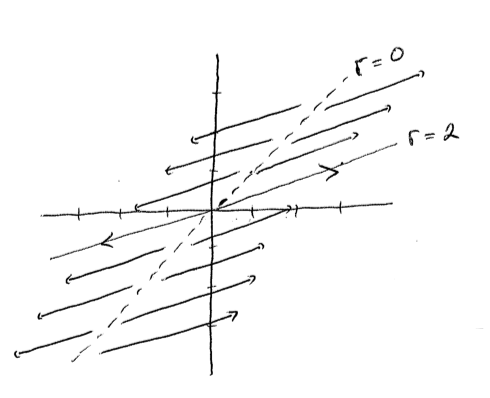
\includegraphics[scale=0.6]{24-5}
	\end{center}
\end{example-N}